\documentclass[12pt]{article}
\usepackage[margin=2.5cm]{geometry}
\usepackage{enumerate}
\usepackage{amsfonts}
\usepackage{amsmath}
\usepackage{fancyhdr}
\usepackage{amsmath}
\usepackage{amssymb}
\usepackage{amsthm}
\usepackage{mdframed}
\usepackage{graphicx}
\usepackage{subcaption}
\usepackage{adjustbox}
\usepackage{listings}
\usepackage{xcolor}
\usepackage{booktabs}
\usepackage[utf]{kotex}
\usepackage{hyperref}
\usepackage{accents}

\definecolor{codegreen}{rgb}{0,0.6,0}
\definecolor{codegray}{rgb}{0.5,0.5,0.5}
\definecolor{codepurple}{rgb}{0.58,0,0.82}
\definecolor{backcolour}{rgb}{0.95,0.95,0.92}

\lstdefinestyle{mystyle}{
    backgroundcolor=\color{backcolour},
    commentstyle=\color{codegreen},
    keywordstyle=\color{magenta},
    numberstyle=\tiny\color{codegray},
    stringstyle=\color{codepurple},
    basicstyle=\ttfamily\footnotesize,
    breakatwhitespace=false,
    breaklines=true,
    captionpos=b,
    keepspaces=true,
    numbers=left,
    numbersep=5pt,
    showspaces=false,
    showstringspaces=false,
    showtabs=false,
    tabsize=1
}

\lstset{style=mystyle}

\pagestyle{fancy}
\renewcommand{\headrulewidth}{0.4pt}
\lhead{CSC 343}
\rhead{Worksheet 12 Solution}

\begin{document}
\title{CSC343 Worksheet 12 Solution}
\maketitle

\begin{enumerate}[1.]
    \item

    \begin{itemize}
        \item Keys
        \begin{itemize}
            \item $\{$id of molecule$\}$
            \item $\{$x position, y position, z position$\}$
        \end{itemize}
        \item Functional Dependencies
        \begin{enumerate}[1.]
            \item id of molecule $\to$ x position, y position, z position, x velocity, y velocity, z velocity
            \item x position, y position, z position $\to$ id of molecule, x velocity, y velocity, z velocity
        \end{enumerate}
    \end{itemize}

    \bigskip

    \underline{\textbf{Notes:}}

    \bigskip

    \begin{itemize}
        \item Function Dependencies
        \begin{itemize}
            \item \textit{Functional Dependency} is a relationship between two attributes
            typically between the key and other non-key attributes within a table.

            \bigskip

            \underline{\textbf{Example:}}

            \bigskip

            $\text{SIN} \to \text{Name, Address, Birthdate}$

            \bigskip

            \underline{\textbf{Example 2:}}

            \bigskip

            $\textbf{ISBN} \to \text{Title}$

        \end{itemize}

        \item Key of Relations
        \begin{itemize}
            \item One or more attributes $\{A_1,A_2,...,A_n\}$ is a key for a relation R if
            \begin{enumerate}[1.]
                \item Those attributes functionally determine all other attributes of the relation
                \item No proper subset of $\{A_1,A_2,...A_n\}$ functionally determines all other attributes of R


                \bigskip

                \underline{\textbf{Example:}}

                \bigskip

                Given relation

                \bigskip

                $R = \text{Movies1(title, year, length, genre, studioName, starName)}$

                \begin{enumerate}
                    \item $\{$title, year, starName $\}$ form a key for the relation \textbf{Movies1}
                    \item $\{$ year, starName $\}$ is not a key. Same star can be in multiple
                    movies per year
                \end{enumerate}
            \end{enumerate}

            \item Superkeys
            \begin{itemize}
                \item Means a a set of attributes that contains a key
                \item Don't need to be minimal

                \bigskip

                \underline{\textbf{Example:}}

                Given relation

                \bigskip

                $R = \text{Movies1(title, year, length, genre, studioName, starName)}$

                \begin{itemize}
                    \item $\{$ title, year, starName $\}$ is a key and superkey
                    \item $\{$ title, year, starName, title, year, length$\}$ is a superkey
                \end{itemize}
            \end{itemize}
        \end{itemize}
    \end{itemize}

    \bigskip

    \underline{\textbf{References:}}

    \bigskip

    \begin{enumerate}[1)]
        \item OpenTextBC, Chapter 11 Functional Dependencies, \href{https://opentextbc.ca/dbdesign01/chapter/chapter-11-functional-dependencies/#:~:text=A%20functional%20dependency%20(FD)%20is,determines%20the%20value%20of%20Y.}{link}
    \end{enumerate}

    \item

    \begin{enumerate}[a)]

        \item

        \begin{enumerate}[1.]
            \item $AB \to C$
            \item $AB \to D$
            \item $C \to A$
            \item $C \to B$
            \item $D \to B$
            \item $D \to C$
            \item $C \to D$
            \item $D \to A$
        \end{enumerate}

        \bigskip

        \begin{mdframed}
            \underline{\textbf{Second Attempt:}}

        $\{A,B\}^+ = \{A,B,C,D\}$, so the following non-trivial FDs follows:
        $AB \to C$ and $AB \to D$.

        \bigskip

        $\{C\}^+ = \{D,A\}$, so the following non-trivial FDs follows
        $C \to D$ and $C \to A$.

        \bigskip
        $\{D\}^+ = \{A\}$, so the following non-trivial FDs follows:
        $D \to A$.


        \end{mdframed}

        \bigskip

        \underline{\textbf{Notes:}}

        \bigskip

        \begin{itemize}
            \item The Splitting / Combining Rule
            \begin{itemize}
                \item Combining Rule
                \begin{itemize}
                    \item

                    $A_1,A_2,\cdots,A_n \to B_i$ for $i = 1,2,...,m$

                    to

                    $A_1,A_2,\cdots A_n \to B_1,B_2,\cdots B_m$
                \end{itemize}

                \bigskip

                \underline{\textbf{Example:}}

                \bigskip

                Given

                \bigskip

                title year $\to$ length

                title year $\to$ genre

                title year $\to$ studioName

                \bigskip

                it's combined form is

                \bigskip

                title year $\to$ length genre studioName

                \bigskip

                \item Splitting Rule
                \begin{itemize}
                    \item
                    \item

                    $A_1,A_2,\cdots A_n \to B_1,B_2,\cdots B_m$

                    to

                    $A_1,A_2,\cdots,A_n \to B_i$ for $i = 1,2,...,m$

                \end{itemize}

                \bigskip

                \underline{\textbf{Example:}}

                \bigskip

                Given

                \bigskip

                title year $\to$ length

                \bigskip

                It's splitted form is

                \bigskip

                title $\to$ length

                year $\to$ length
            \end{itemize}

            \item Trivial Functional Dependencies

            \bigskip

            \begin{itemize}
                \item A functional dependency $FD: X \to Y$ is \textbf{trivial}
                if $Y$ is a subset of $X$

                \bigskip

                \underline{\textbf{Exmaple:}}

                \bigskip

                title year $\to$ title

                \bigskip

                \underline{\textbf{Example 2:}}

                \bigskip

                title $\to$ title

            \end{itemize}

            \item Non-trivial Functional Dependencies
            \begin{itemize}
                \item is a case where some but not all of the attributes on the R.H.S
                of an FD are also on L.H.S

                \bigskip

                \underline{\textbf{Example:}}

                \bigskip

                title year $\to$ title movieLength

                \bigskip

                \item Can be simplified using \textbf{tirivial-dependency rule}
                \begin{itemize}
                    \item The $FD$ $A_1A_2 \cdots A_n \to B_1B_2 \cdots B_m$ is equivalent to

                    $A_1 A_2 \cdots A_n \to C_1 C_2 \cdots C_k$

                    \bigskip

                    where $C$'s are all those $B$'s that are not in $A$'s.


                    \begin{center}
                    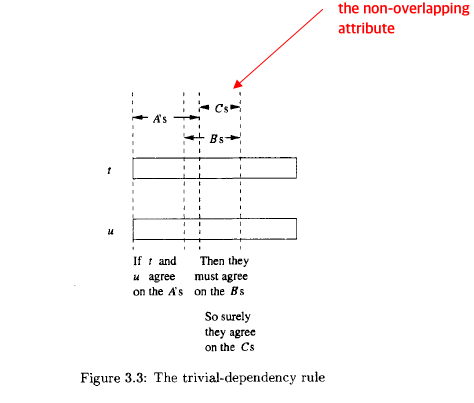
\includegraphics[width=\linewidth]{images/worksheet_12_solution_1.png}
                    \end{center}
                \end{itemize}
            \end{itemize}

            \item Computing the Clousre of Attributes
            \begin{itemize}
                \item Closure of attribute set $\{X\}$ is denoted as $\{X\}^+$.
                \item The closure means a given set of attributes $A$ satisfying FD, are a sets of all attributes
                $B$ such that $A \to B$

                \bigskip

                \underline{\textbf{Example:}}

                \bigskip


                Given attributes $A,B,C,D,E,F$ and FDs $AB \to C$, $BC \to AD$, $D \to E$
                and $CF \to B$, What is the closure of $\{A,B\}$ or $\{A,B\}^+$

                \bigskip

                \begin{enumerate}[1.]
                    \item Start with $\{A,B\}$.
                    \item Split $BC \to AD$
                    \begin{itemize}
                        \item We have $BC \to A$ and $BC to D$
                        \item Since $A$ is in $\{A,B\}$, this is not included
                        \item Since $D$ is not in  $\{A,B\}$, this IS included

                        \bigskip

                        So, we have $\{A,B,D\}$
                    \end{itemize}
                    \item Since $C$ in $AB \to C$ is NOT in $\{A,B,C,D\}$, $C$ is included and we have $\{A,B,C,D\}$
                    \item Since $A$ in $BC \to A$ is in $\{A,B,C,D\}$, this is skipped
                    \item Since $E$ is not in $D \to E$, $E$ is included and we have $\{A,B,C,D,E\}$
                    as our solution
                \end{enumerate}
            \end{itemize}

            \item Why the Closure Algorithm Works
            \item Transitive Rule
            \begin{itemize}
                \item Definition

                \bigskip

                If $A_1A_2 \cdots A_n \to B_1B_2 \cdots B_m$ and $B_1B_2 \cdots B_m \to C_1C_2 \cdots C_k$
                hold in relation $R$, $A_1A_2 \cdots A_n \to C_1C_2 \cdots C_k$ also holds in $R$.

                \bigskip

                \underline{\textbf{Example:}}

                \bigskip

                Given

                \bigskip

                title year $\to$ studioName

                studioName $\to$ studioAddr

                \bigskip

                Transitive rule says the above is equal to the following

                \bigskip

                title year $\to$ studioAddr

            \end{itemize}

            \item Inference Rules
            \begin{itemize}
                \item Is allso called \textbf{Armstrong's Axioms}
                \item Has 3 axioms
                \begin{enumerate}[1.]
                    \item \textit{Reflexivity}
                    \begin{itemize}
                        \item If $\{B_1, B_2, ..., B_n\} \subseteq \{A_1, A_2, ..., A_n\}$ then

                        $A_1A_2 \cdots  A_n \to B_1B_2 \cdots B_m$
                        \item also called \textbf{trivial FDs}
                    \end{itemize}
                    \item \textit{Augmentation}
                    \begin{itemize}
                        \item If $A_1A_2 \cdots A_n \to B_1B_2 \cdots B_m$

                        then $A_1A_2 \cdots A_nC_1C_2 \cdots C_k \to B_1B_2 \cdots B_m C_1C_2 \cdots C_k$

                        \item $ C_1C_2 \cdots C_k$ are any set of attributes
                    \end{itemize}
                    \item \textit{Transitivity}
                    \begin{itemize}
                        \item If $A_1A_2 \cdots A_n \to B_1B_2 \cdots B_m$ and $B_1B_2 \cdots B_m \to C_1C_2 \cdots C_k$

                        then $A_1A-2 \cdots A_n \to C_1C_2 \cdots C_k$

                    \end{itemize}
                \end{enumerate}
            \end{itemize}
        \end{itemize}

        \item

        ${A,B}$ is the only key of $R$.

        \bigskip

        \underline{\textbf{Notes:}}

        \bigskip

        \begin{itemize}
            \item Key of Attributes
            \begin{itemize}
                \item \textbf{Definition:} A set of attributes $\{A_1,A_2,\cdots,A_n\}$
                is a key for a relation $R$ if


                \begin{enumerate}[1.]
                    \item Those attributes functionally determine all other attributes
                    \item No proper subset of $\{A_1, A_2, ..., A_n\}$ functionally determines all other attributes
                    of $R$.
                \end{enumerate}
            \end{itemize}
        \end{itemize}

        \item

        The superkeys that are not keys are: $\{A,B,C\}$, $\{A,B,D\}$, $\{A,B,C,D\}$
    \end{enumerate}

    \item

    \begin{enumerate}[i)]
        \item

        \begin{enumerate}[a)]
            \item

            \bigskip

            $\{A\}^+ = \{A,B,C,D\}$, so we have $A \to A$, $A \to B$, $A \to C$, $A \to D$

            \bigskip

            $\{B\}^+ = \{C,D\}$, so we have $B \to C$ and $B \to D$

            \item

            $\{A\}$ is the key of $S$.

            \item

            The super keys that are not keys are:

            \bigskip

            $\{A,B\}$, $\{A,C\}$, $\{A,D\}$, $\{A,B,C\}$, $\{A,B,D\}$, $\{A,B,C,D\}$
        \end{enumerate}

        \item

        \begin{enumerate}[a)]
            \item

            \bigskip

            $\{A\}^+ = \{A\}$, so this FD is trivial.

            \bigskip

            $\{B\}^+ = \{B\}$, so this FD is trivial.

            \bigskip

            $\{C\}^+ = \{C\}$, so this FD is trivial.

            \bigskip

            $\{D\}^+ = \{D\}$, so this FD is trivial.

            \bigskip

            $\{A,B\}^+ = \{A,B,C,D\}$, so we have $AB \to A$, $AB \to B$, $AB \to C$, $AB \to D$

            \bigskip

            $\{A,C\}^+ = \{A,C\}$, so we have $AC \to A$, $AC \to C$

            \bigskip

            $\{A,D\}^+ = \{A,D,B\}$, so we have $AD \to A$, $AD \to D$, $AD \to B$

            \bigskip

            $\{B,C\}^+ = \{B,C,D,A\}$, so we have $BC \to A$, $BC \to B$, $BC \to C$, $BC \to D$

            \bigskip

            $\{D,C\}^+ = \{D,C,A,B\}$, so we have $DC \to D$, $DC \to C$, $DC \to A$, $DC \to B$

            \bigskip

            $\{A,B,C\}^+ = \{A,B,C,D\}$, so we have $ABC \to A$, $ABC \to B$, $ABC \to C$, $ABC \to D$

            \bigskip

            $\{B,C,D\}^+ = \{B,C,D,A\}$, so we have $BCD \to A$, $BCD \to B$, $BCD \to C$, $BCD \to D$

            \bigskip

            $\{C,D,A\}^+ = \{C,D,A,B\}$, so we have $CDA \to A$, $CDA \to B$, $CDA \to C$, $CDA \to D$

            \bigskip

            $\{D,A,B\}^+ = \{D,A,B,C\}$, so we have $DAB \to A$, $DAB \to B$, $DAB \to C$, $DAB \to D$

            \bigskip

            $\{D,A,B\}^+ = \{D,A,B,C\}$, so we have $DAB \to A$, $DAB \to B$, $DAB \to C$, $DAB \to D$

            \bigskip

            $\{A,B,C,D\}^+ = \{A,B,C,D\}$, so this FD is trivial.

            \item

            $\{A,B\}$, $\{A,C\}$, $\{B,C\}$, $\{D,C\}$ are the keys of $T$.

            \bigskip

            \item

            The super keys that are not keys are:

            \bigskip

            $\{A,B,C\}$, $\{A,B,D\}$, $\{B,C,D\}$, $\{A,D,C\}$, $\{A,B,D\}$, $\{A,B,C,D\}$

        \end{enumerate}

        \item

        \begin{enumerate}[a)]
            \item

            $\{A\}^+ = \{A,B,C,D\}$, so we have $A \to C$, $A \to D$

            \bigskip

            $\{B\}^+ = \{A,B,C,D\}$, so we have $B \to A$, $B \to D$

            \bigskip

            $\{C\}^+ = \{A,B,C,D\}$, so we have $C \to A$, $C \to B$

            \bigskip

            $\{D\}^+ = \{A,B,C,D\}$, so we have $D \to B$, $D \to C$

            \bigskip

            $\{A,B\}^+ = \{A,B,C,D\}$, so we have $AB \to C$, $AB \to D$

            \bigskip

            $\{B,C\}^+ = \{A,B,C,D\}$, so we have $BC \to A$, $BC \to D$

            \bigskip

            $\{B,D\}^+ = \{A,B,C,D\}$, so we have $BD \to A$, $BD \to C$

            \bigskip

            $\{C,D\}^+ = \{A,B,C,D\}$, so we have $CD \to A$, $CD \to B$

            \bigskip

            $\{C,D\}^+ = \{A,B,C,D\}$, so we have $CD \to A$, $CD \to B$

            \bigskip

            $\{A,B,C\}^+ = \{A,B,C,D\}$, so we have $ABC \to D$

            \bigskip

            $\{B,C,D\}^+ = \{A,B,C,D\}$, so we have $BCD \to A$

            \bigskip

            $\{C,D,A\}^+ = \{A,B,C,D\}$, so we have $CDA \to B$

            \bigskip

            $\{D,A,B\}^+ = \{A,B,C,D\}$, so we have $DAB \to C$

            \item

            $\{A\},\{B\},\{C\},\{D\}$ are the keys of $U$.

        \end{enumerate}


    \end{enumerate}
\end{enumerate}

\end{document}